\documentclass[10pt, letterpaper]{article}
\usepackage[cm]{fullpage}
\usepackage{algpseudocode}
\usepackage{algorithm}
\usepackage{graphicx}
\usepackage[section]{placeins}
\usepackage[table]{xcolor}
\usepackage{amsmath}
\usepackage[margin=0.7in]{geometry}

\algrenewcommand\Return{\State \algorithmicreturn{} }%

\title{0-1 Knapsack}
\author{Daiwei Chen \and Joseph Watts}

\begin{document}
\maketitle
	\begin{abstract}
	0-1 Knapsack is used a ton, seriously. Look it up.
	\end{abstract}

\section{Background and Related Work}
	0-1 Knapsack deals with xyz and is important to its real world use cases. One such use is abc.
\section{Greedy Algorithm}

\section{Dynamic Algorithm}

\section{Experimental Setup}

\section{Results}
	% Diagram showing the average time between different approaches
	\begin{figure}[htbp]
		\begin{center}
			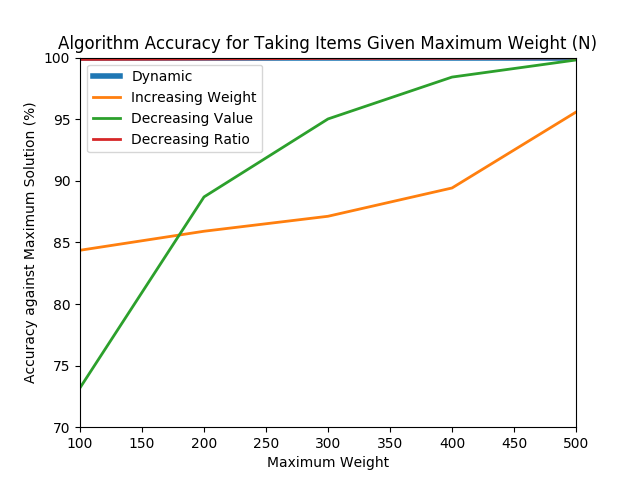
\includegraphics[width=0.70\textwidth]{python/accuracyGraph.png}
			\caption{Algorithm Accuracy for Taking Items Given Maximum Weight $n$}
			\label{fig:accuracy-graph}
		\end{center}
	\end{figure}
	% Diagram showing the % accuracy of different approaches
	\begin{figure}[htbp]
		\begin{center}
			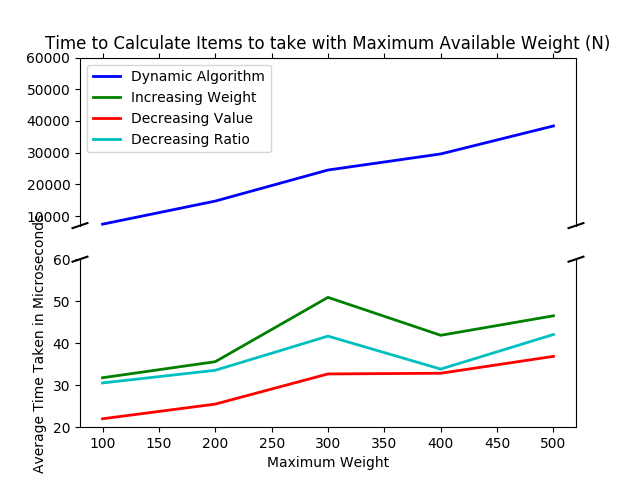
\includegraphics[width=0.70\textwidth]{python/timeGraph.png}
			\caption{Time to Calculate Items to take with Maximum Available Weight $n$}
			\label{fig:time-graph}
		\end{center}
	\end{figure}
\section{Conclusions}

\end{document}
